 \begin{activity} \label{A:10.2.10} Consider the function $f$ defined by 
   $$
   f(x,y) = \frac{xy^2}{x+1}
   $$
   at the point $(1,2)$.

   \ba
   \item Write the trace $f(x,2)$ at the fixed value $y=2$.   
     On the left side of Figure \ref{F:10.2.activity.trace},
     draw the graph of the trace with $y=2$ indicating the scale and
     labels on the axes.  Also, sketch 
     the tangent line at the point $x=1$.

   \begin{figure}[ht]
     \begin{center}
       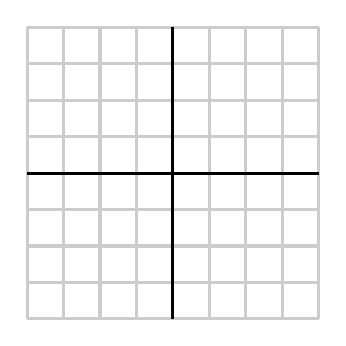
\includegraphics{figures/fig_10_2_empty.eps}
       \hspace*{0.5in}
       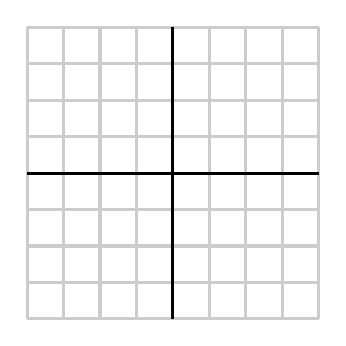
\includegraphics{figures/fig_10_2_empty.eps}
     \end{center}
     \caption{Traces of $f(x,y) = \frac{xy^2}{x+1}$.}
     \label{F:10.2.activity.trace}
   \end{figure}

   \item Find the partial derivative $f_x(1,2)$ and relate its value
     to the sketch you just made.

   \item Write the trace $f(1,y)$ at the fixed value $x=1$.  
     On the right side of Figure \ref{F:10.2.activity.trace},
     draw the graph of the trace with $x=1$ indicating the scale and
     labels on the axes.  Also, sketch 
     the tangent line at the point $y=2$.

   \item Find the partial derivative $f_y(1,2)$ and relate its value
     to the sketch you just made.


   \ea


\end{activity}

\begin{activitySolution}
\ba
\item Here we have $f(x,2) = \frac{4x}{x+1}$. At the point where $x=1$, the tangent line to this trace has slope $\frac{d}{dx} f(x,2) \left. \right|_{x=1} = 1$, and so the line tangent to the graph of this trace at $x=1$ has equation $z=2+(x-1)$. 
\item Now $f_x(x,y) = \frac{(x+1)(y^2) - xy^2}{(x+1)^2}$, and so $f_x(1,2) = \frac{8-4}{4} = 1$. This is the slope of the line tangent to the trace $f(x,2)$ at the point where $x=1$, as calculated in part (a). 
\item Here we have $f(1,y) = \frac{1}{2}y^2$. At the point where $y=2$, the tangent line to this trace has slope $\frac{d}{dy} f(1,y) \left. \right|_{y=2} = 2$, and so the line tangent to the graph of this trace at $y=2$ has equation $z=2+2(y-2)$. 
\item Now $f_y(x,y) = \frac{x}{x+1}(2y)$, and so $f_y(1,2) = 2$. This is the slope of the line tangent to the trace $f(1,y)$ at the point where $y=2$, as calculated in part (c).  
\ea
\end{activitySolution}

\aftera
